\section{Sprint Material} % (fold)
\label{sec:Sprint Material}
\subsection{Version} % (fold)
\label{sub:Version}
The current state of our app has version 0.0.1. Meaning that the app is still alpha quality, with some functionality implementet, ot of unfinished work.
% subsection Version (end)
\subsection{Source code} % (fold)
\label{sub:Source code}
We still use Git and GitHub. The source code is available at: \url{https://github.com/mundane/ETA_analytics}, in the app folder. The other folders contains prototypes and experiments.
% subsection Source code (end)
\subsection{Sprint Explanation}
The burndown chart shows that, better coordination on task and work assignment helped in completing the taks planned for this sprint.
Surplus time was spent on research for eg Tools for Software Documentation and architecture descriptonal standard,this have been cumlatively added in the sprint burndown.
%\begin{figure}[h!]
%  \centering
%    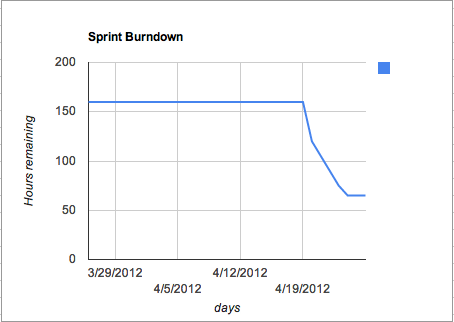
\includegraphics[width=0.8\textwidth]{images/burndown.png}
%	\caption{Burndown chart for sprint \# 2. Easter holidays and exams is the reason for the steep curve.}
%\end{figure}
The project backlog and the graph with the hours we spent are at the end of this document in appendix \ref{sec:Scrum Material}. The reader should note that the graph are vector graphics, so zooming is posible. \\
As can be seen from our backlog we have added some user stories and kept on working on some from the previous sprint.
\subsection{User Stories}
For sprint \# 3 we had the following user stories: \\
As an analytic \\
I want to be able to browse files on the devices\\
So that I can view my files on the App \\

As a programmer\\
I want to have my project source code commented  \\
So that I can get a better overview \\

As an software architect\\
I want a the Application documented with arcitectural diagrams \\
So that I can get a better overview of the functionalities\\

As a developer\\
I want to compress code for better performance\\
So I can speed up the load time to seconds\\

As a developer\\
I want to remove dead code and optimize my source code\\
So I fucntionalities more efficient\\

As a developer\\
I want to remove dead code and optimize my source code\\
So I functionalities efficient\\


\subsection{Tasks} % (fold)
\label{sub:Tasks}
We divided the stories up in the following tasks
% subsection Tasks (end)Tasks
\begin{itemize}
	\item Implement File Browser.
	\item Research Phonegap and its standard API. 
	\item Javascript documentation tool and its core aspects.
	\item Closure Javascript source code optimizer.
	\item Improve testing scenarios and leftovers from sprint2
\end{itemize}










% section Sprint Material (end)
